%%%% Paramétrage du TD %%%%
\def\xxactivite{ \ifprof \normalsize{Activation 1 -- Corrigé } \else  \ifcolle Colle \else Activation 1\fi \fi} % \normalsize \vspace{-.4cm}
\def\xxauteur{\textsl{Xavier Pessoles}}


\def\xxnumchapitre{Chapitre 1 \vspace{.2cm}}
\def\xxchapitre{\hspace{.12cm} Approche énergétique}

\def\xxcompetences{%
\footnotesize{
\textsl{%
\textbf{Savoirs et compétences :}\\
\vspace{-.2cm}
\begin{itemize}[label=\ding{112},font=\color{ocre}] 
\item Mod2.C18.SF1 : Déterminer l’énergie cinétique d’un solide, ou d’un ensemble de solides, dans son mouvement par rapport à un autre solide.
\item Res1.C1.SF1 : Proposer une démarche permettant la détermination de la loi de mouvement.
%\item Mod1.C5.SF2 : Déterminer la puissance des actions mécaniques extérieures à un solide ou à un ensemble de solides, dans son mouvement rapport à un autre solide.
%\item Mod1.C5.SF3 : Déterminer la puissance des actions mécaniques intérieures à un ensemble de solides.
\end{itemize}}}}


\def\xxtitreexo{Activation -- Système de dépose de composants électroniques}%Motorisation du moteur Haibike}
\def\xxsourceexo{\hspace{.2cm} \footnotesize{Émilien Durif -- E3A PSI 2011}}

\def\xxfigures{
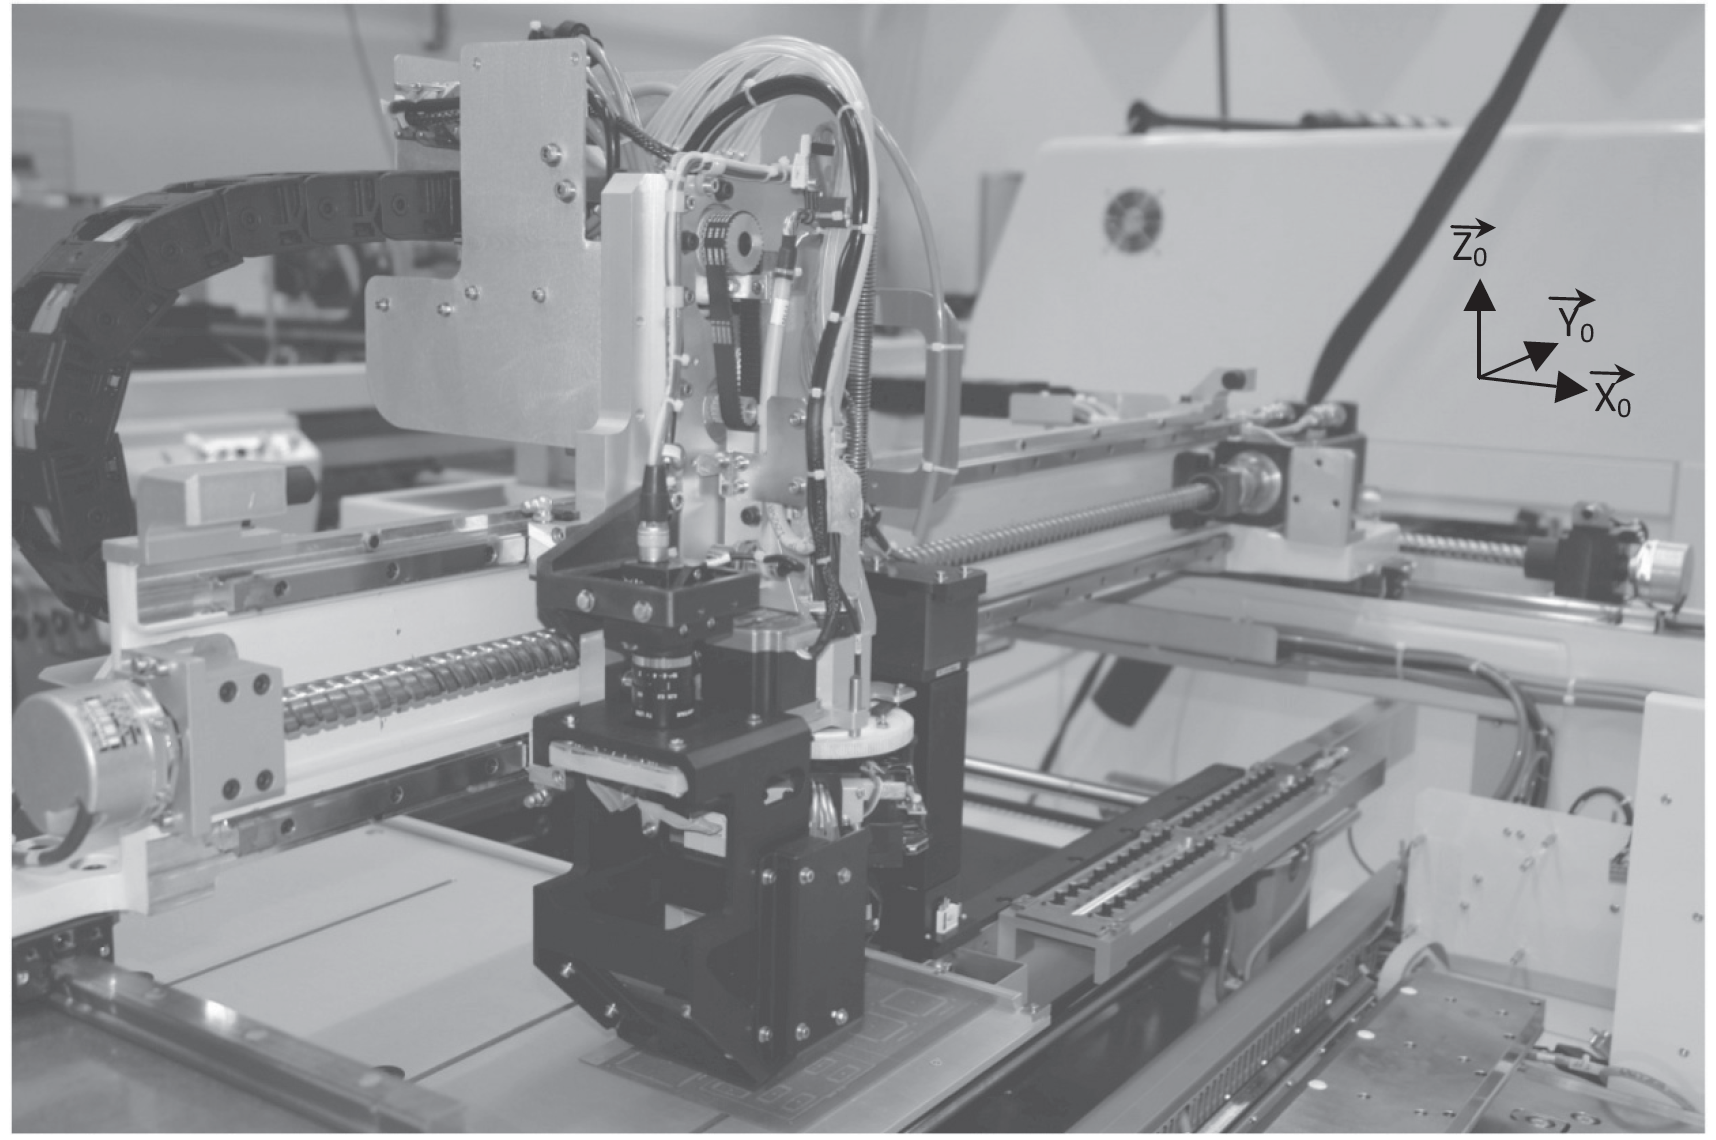
\includegraphics[width=.7\linewidth]{axe_y_photo}
}%figues de la page de garde

\input{\repRel/Style/pagegarde_TD}
\setcounter{numques}{0}

\setlength{\columnseprule}{.1pt}

\pagestyle{fancy}
\thispagestyle{plain}


\vspace{5.2cm}

\def\columnseprulecolor{\color{ocre}}
\setlength{\columnseprule}{0.4pt} 

%%%%%%%%%%%%%%%%%%%%%%%

\setcounter{exo}{0}

\ifprof
%\begin{multicols}{2}
\else
\begin{multicols}{2}
\fi
\ifprof\else

Le système étudié permet de déposer automatiquement des composants électroniques sur un circuit.
On s'intéresse ici à la modélisation d'un seul axe (selon la direction notée $\overrightarrow{y_0}$) actionné par un moteur électrique et utilisant un mécanisme de transformation de mouvement <<~\textit{vis-écrou}~>>.

\textbf{Hypothèses :}
\begin{itemize}
\item le référentiel associé au repère $R_0=\quadruplet{O_0}{\overrightarrow{x_0}}{\overrightarrow{y_0}}{\overrightarrow{z_0}}$ est supposé galiléen ;
\item les solides seront supposés indéformables ; 
\item on notera $J_1$ le moment d'inertie du solide 1 (composé d'une vis à billes et de l'arbre moteur) selon l'axe $\couple{O_0}{{y_0}}$ : $J_1=I_{\couple{O_0}{{y_0}}}(S_1)$ ;
\item on note $M_3$ et $G_3$ respectivement la masse et le centre d'inertie du solide $S_3$ ;
\item la position de $G_3$ est définie par $\overrightarrow{O_0G_3}=y\cdot \overrightarrow{y_0}+z\cdot \overrightarrow{z_0}$
\item les liaisons sont supposées parfaites (sans jeu ni frottement) sauf la glissière entre $S_0$ et $S_3$ (Coefficient de frottement noté $\mu$) et la pivot entre $S_0$ et $S_1$ (couple résistant noté $C_r$);
\item seul l'action de pesanteur sur $S_3$ sera supposée non négligeable.
\end{itemize}

\ifprof
\else
\begin{center}
%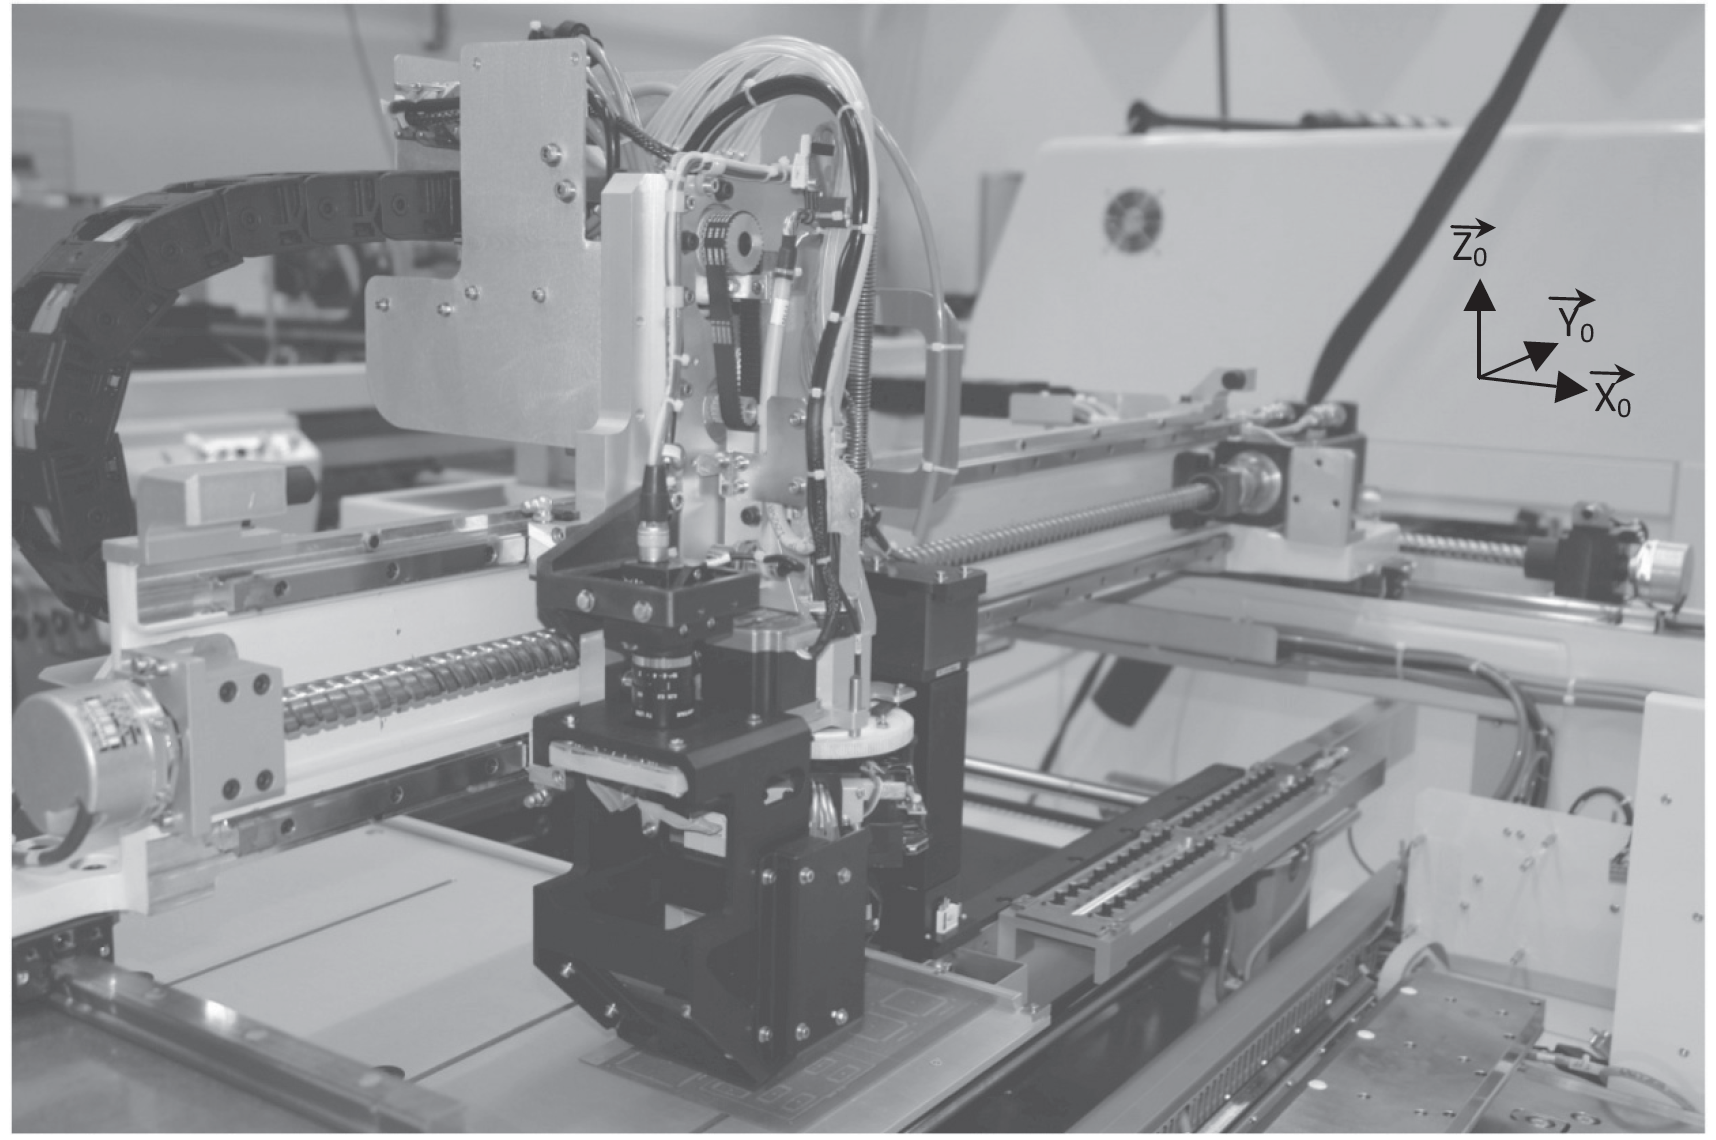
\includegraphics[width=\linewidth]{axe_y_photo.png}

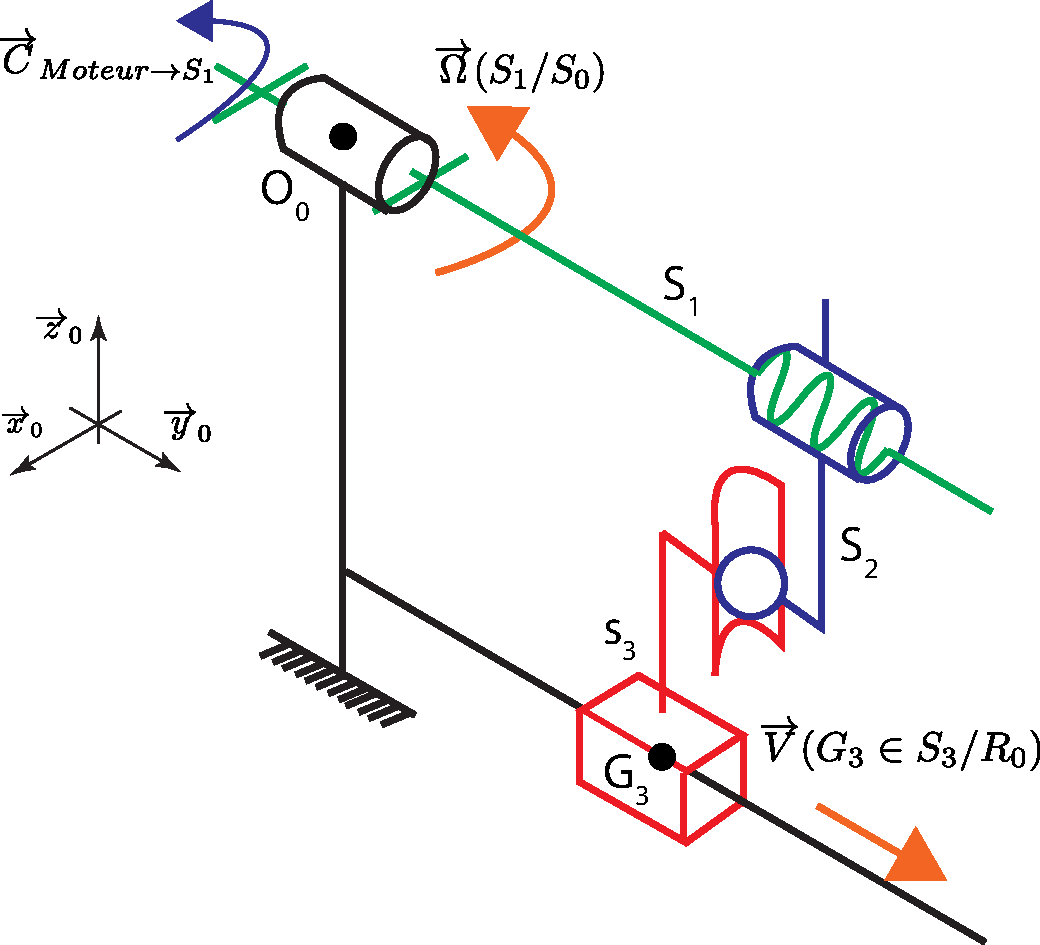
\includegraphics[width=\linewidth]{schema_cine_depose_composant.pdf}

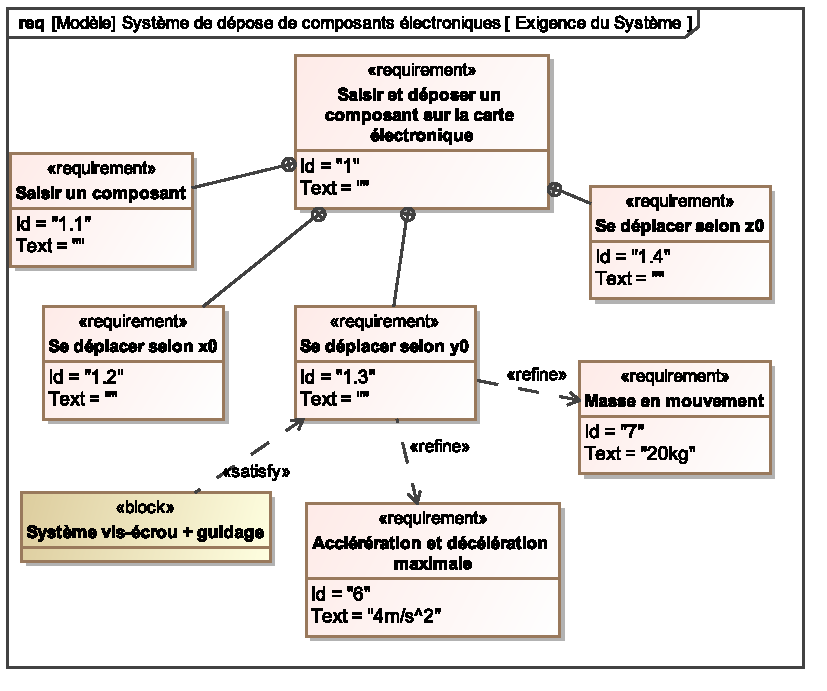
\includegraphics[width=\linewidth]{req_systeme_depose.pdf}
\end{center}
\fi
\begin{itemize}
\item $S_0$ : poutre transversale considérée comme fixe par rapport au bâti.
\item $S_1$ : vis à billes (hélice à droite) et arbre moteur.
\item $S_2$ : écrou de la vis à billes (inertie négligeable).
\item $S_3$ : chariot supportant la tête de dépose (masse $M_3$).
\end{itemize}

\textbf{Données numériques associées au système :}
\begin{itemize}
\item Coefficient de frottement dans la liaison glissière (rail + patin à billes) : $\mu = 0,1$.
\item Pas de la vis à billes : $p = \SI{20}{mm}$.
\item Diamètre de la vis à billes : $D =\SI{25}{mm}$.
\item Moment d'inertie de la vis à billes suivant l'axe $\overrightarrow{y_0}$ : $I_v = 2,15 \times 10^{-4}\;\text{kg m}^2$.
\item Couple résistant sur la vis due à son guidage (paliers + joints): $C_r = \SI{3}{Nm}$.
\item $l$, longueur libre de la vis -- entre deux paliers -- (mm) : $\SI{1000}{mm}$.
\item Caractéristiques du moteur d'axe (puissance, vitesse maxi, inertie) :
\begin{itemize}
\item couple maximal, $C_{\text{max}} = \SI{21,2}{Nm}$;
\item fréquence de rotation maximale, $N_m = \SI{6000}{tr/min}$;
\item moment d'inertie du rotor du moteur suivant l'axe $\overrightarrow{y_0}$, $I_m = 1,6 \times 10^{-4}\;\text{kg m}^2$.
\end{itemize}

\end{itemize}

\clearpage



\begin{obj}
L'objectif de cette étude est de relier les grandeurs liées à l'actionneur du système (moteur) :
\begin{itemize}
\item couple moteur transmis à $S_1$ : $\overrightarrow{C}_{\text{Moteur}\to S_1}\cdot \overrightarrow{y_0}=C_m(t)$ ;
\item vitesse de rotation de $S_1$ : $\overrightarrow{\Omega}(S_1/R_0)\cdot \overrightarrow{y_0}=\dot{\theta}(t)$;
\end{itemize} 
à celles liées à l'effecteur (tête de dépose $S_3$) : 
\begin{itemize}
\item masse : $M_3$;
\item cinématique de $S_3$ : $\overrightarrow{a}(G_3R_0)\cdot \overrightarrow{y_0}=\ddot{y}(t)$.
\end{itemize}
\end{obj}




On considère l'ensemble $E=\left\{S_1+S_2+S_3\right\}$.
\fi

\question{Construire le graphe des liaisons modélisant le système entier.}

\ifprof\begin{corrige}
\begin{center}
%\includegraphics[width=0.9\textwidth]{../../../../sujets/dynamique/depose_composant/images/graph_structure.png}
\end{center}
\end{corrige}\else\fi

\question{Déterminer l'expression de $\mathcal{P}(\text{ext} \rightarrow E/R_g)$ en fonction de puissances extérieures élémentaires (on ne développera pas les calculs explicitement pour l'instant).}
\ifprof\begin{corrige}
\begin{align*}
\mathcal{P}(\text{ext}\rightarrow E/R_g)=\mathcal{P}(S_0 \rightarrow S_1/R_0)+\mathcal{P}(\text{Moteur }\rightarrow S_1/R_0)
+\mathcal{P}(S_0 \rightarrow S_3/R_0)+\mathcal{P}(\text{poids} \rightarrow S_3/R_0)
\end{align*}
\end{corrige}\else\fi


\question{Calculer $\mathcal{P}(\text{ext}\rightarrow E/R_0)$ en fonction des données du problème.}
\ifprof\begin{corrige}
On a : 
$$
\mathcal{P}(\text{ext}\rightarrow E/R_g)=\mathcal{P}(S_0 \rightarrow S_1/R_0)+\mathcal{P}(\text{Moteur}\rightarrow S_1/R_0)
+\mathcal{P}(S_0 \rightarrow S_3/R_0)+\mathcal{P}(\text{poids} \rightarrow S_3/R_0)
$$ 
\begin{itemize}
\item $\mathcal{P}(S_0 \rightarrow S_1/R_0)=\torseurstat{T}{S_0}{S_1}\otimes \torseurcin{V}{S_1}{R_0}$
$=\torseurl{X_{01}\cdot \overrightarrow{x_0}+Y_{01}\cdot \overrightarrow{y_0}+Z_{01}\cdot \overrightarrow{z_0}}{L_{01}\cdot \overrightarrow{x_0} \pm C_r\cdot \overrightarrow{y_0}+N_{01}\cdot \overrightarrow{z_0}}{O_0}
\otimes
\torseurl{\dot{\theta}(t)\cdot \overrightarrow{y_0}}{\overrightarrow{0}}{O_0}$
$=\pm C_r\cdot \dot{\theta}(t)$. 
Le signe de la composante suivant $\overrightarrow{y_0}$ dépendra du sens du mouvement de $S_1/S_0$.
\item $\mathcal{P}(\text{Moteur} \rightarrow S_1/R_0)$ $=\torseurstat{T}{\text{Moteur}}{S_1}\otimes \torseurcin{V}{S_1}{R_0}$
$=\torseurl{\overrightarrow{0}}{C_m\cdot \overrightarrow{y_0}}{-}
\otimes
\torseurl{\dot{\theta}(t)\cdot \overrightarrow{y_0}}{\overrightarrow{0}}{O_0}$
$=C_m\cdot \dot{\theta}(t)$.
\item $
\mathcal{P}(S_0 \rightarrow S_3/R_0)$ $=\torseurstat{T}{S_0}{S_3}\otimes \torseurcin{V}{S_3}{R_0}$
$=\torseurl{X_{03}\cdot \overrightarrow{x_0}\pm Y_{03}\cdot \overrightarrow{y_0}+Z_{03}\cdot \overrightarrow{z_0}}{L_{03}\cdot \overrightarrow{x_0} + M_{03}\cdot \overrightarrow{y_0}+N_{03}\cdot \overrightarrow{z_0}}{-}
\otimes
\torseurl{\overrightarrow{0}}{\dot{y}(t)\cdot \overrightarrow{y_0}}{-}$
$=\pm Y_{03}\cdot \dot{y}(t)$.
\item $\mathcal{P}(\text{Poids} \rightarrow S_3/R_0) $
%$\mathcal{P}(S_0 \rightarrow S_3/R_0)$ 
$=\torseurstat{T}{\text{pes}}{S_3}\otimes \torseurcin{V}{S_3}{R_0}$
 $=\torseurl{\overrightarrow{0}}{-M_3\cdot g\cdot \overrightarrow{z_0}}{G_3}
\otimes
\torseurl{\overrightarrow{0}}{\dot{y}(t)\cdot \overrightarrow{y_0}}{G_3}=0$.
\end{itemize}

$$\mathcal{P}(\text{ext}\rightarrow E/R_0)=\left(C_m\pm C_r\right)\cdot \dot{\theta}(t)\pm Y_{03}\cdot \dot{y}(t)$$
\end{corrige}\else\fi



\question{Calculer l'ensemble des puissances des actions mutuelles dans les liaisons pour l'ensemble $E$ : $\mathcal{P}_{\text{int}}(E)$.}
\ifprof\begin{corrige}
\begin{itemize}
\item D'après le graphe des liaisons : $
\mathcal{P}_{\text{int}}(E)=\mathcal{P}(S_1 \leftrightarrow S_2)+\mathcal{P}(S_2 \leftrightarrow S_3)$.
\item Calcul de $\mathcal{P}(S_1 \leftrightarrow S_2)=$
$=\torseurstat{T}{S_1}{S_2}\otimes \torseurcin{V}{S_2}{S_1}$
$=\torseurl{X_{12}\overrightarrow{x_0}+Y_{12}\overrightarrow{y_0}+Z_{12}\overrightarrow{z_0}}{L_{12}\overrightarrow{x_0}+M_{12}\overrightarrow{y_0}+N_{12}\overrightarrow{z_0}}{O_0}
\otimes
\torseurl{q_{21}\overrightarrow{y_0}}{v_{12}\cdot \overrightarrow{y_0}}{O_0}$
$=Y_{12}\cdot v_{12}+q_{21}\cdot M_{12}$.
Or,$
\left\{
\begin{array}{c}
M_{12}=-\frac{p}{2\pi}Y_{12}\\
v_{12}=\frac{p}{2\pi}q_{21}
\end{array}
\right.
$. 
D'où : 
$
\mathcal{P}(S_1 \leftrightarrow S_2)
=Y_{12}\cdot v_{12}+q_{21}\cdot M_{12}=\frac{p}{2\pi}\left[Y_{12}\cdot q_{21}-q_{21}\cdot Y_{12}\right]=0
$.

\item Calcul de $\mathcal{P}(S_2 \leftrightarrow S_3)=$
$
\torseurstat{T}{S_2}{S_3}\otimes \torseurcin{V}{S_3}{S_2}$
$=\torseurl{A}{X_{23}\overrightarrow{x}_0+Y_{23}\overrightarrow{y_0}}{\overrightarrow{0}}
\otimes
\torseurl{A}{p_{32}\overrightarrow{x}_0+q_{32}\overrightarrow{y}_0+r_{32}\overrightarrow{z_0}}{w_{32}\cdot \overrightarrow{z_0}}\\
=0$.

\item On en déduit donc : 
$
\mathcal{P}_{\text{int}}(E)=0$.
\end{itemize}

\end{corrige}\else\fi



\question{Déterminer l'énergie cinétique de l'ensemble $E$ dans son mouvement par rapport à $R_0$}
\ifprof\begin{corrige}
\begin{itemize}
\item Énergie cinétique de l'ensemble dans son mouvement par rapport à $R_0$ : 
$$
E_c(E/R_0)=E_c(1/R_0)+E_c(2/R_0)+E_c(3/R_0)
$$

\item Énergie cinétique de 1 dans son mouvement par rapport à $R_0$ :
$E_c(1/R_0)
=\dfrac{1}{2}
\torseurci{1}{R_0}
\otimes \torseurcin{V}{1}{R_0}$
$=\frac{1}{2}\torseurl{\overrightarrow{*}}{\overline{\overline{I}}_{O_0}(S_1)\cdot \dot{\theta}(t)\overrightarrow{y_0}}{O_0}\otimes
 \torseurl{\dot{\theta}(t)\overrightarrow{y_0}}{\overrightarrow{0}}{O_0}$
$=\frac{1}{2}\left[\dot{\theta}^2\overline{\overline{I}}_{O_0}(S_1)\cdot \overrightarrow{y}_0\cdot \overrightarrow{y}_0\right]$
$=\frac{1}{2}J_1\cdot \dot{\theta}^2=\frac{1}{2}\left(I_m+I_v\right)\cdot \dot{\theta}^2$.

\item Énergie cinétique de 2 dans son mouvement par rapport à $R_0$ : $
E_c(2/R_0)=\frac{1}{2}\torseurci{2}{R_0}\otimes \torseurcin{V}{2}{R_0}
=0$
car l'inertie de 2 est négligeable.
 
\item Énergie cinétique de 3 dans son mouvement par rapport à $R_0$ :$
E_c(3/R_0)=\frac{1}{2}\torseurci{3}{R_0}\otimes \torseurcin{V}{3}{R_0}
=\torseurl{-}{M_3\cdot \dot{y}(t)\cdot \overrightarrow{y_0}}{\overrightarrow{0}}\otimes
 \torseurl{-}{\overrightarrow{0}}{\dot{y}(t)\cdot\overrightarrow{y_0}}$ $ =\frac{1}{2}M_3\cdot \dot{y}^2(t)$.
 
\item L'énergie cinétique galiléenne de l'ensemble $E$ :
$E_c(E/R_0)=\frac{1}{2}\left[\left(I_m+I_v\right)\cdot \dot{\theta}^2(t)+ M_3\cdot \dot{y}^2(t)\right]$.
\end{itemize}
\end{corrige}\else\fi




\question{Déterminer la mobilité du système.}
\ifprof\begin{corrige}
Ici la mobilité vaut 1.
\end{corrige}\else\fi

\question{Déterminer une relation entre les paramètres cinématiques du problème.}

\ifprof\begin{corrige}
Par une fermeture cinématique on pourrait montrer : $
\dot{y}(t)=-\frac{p}{2\pi}\dot{\theta}(t).
$
\end{corrige}\else\fi

\question{Déterminer l'inertie équivalente de $E$ ramenée à la rotation autour de l'axe $\couple{O_0}{{y_0}}$ et du paramètre $\dot{\theta}(t)$.}

\ifprof\begin{corrige}
$E_c(E/R_0)=\frac{1}{2}\left[\left(I_m+I_v\right)\cdot \dot{\theta}^2(t)+ M_3\cdot \dot{y}^2(t)\right]
=\frac{1}{2}\left[\left(I_m+I_v\right)+ M_3\cdot \left(\frac{p}{2\pi}\right)^2\right]\cdot \dot{\theta}^2(t)$
d'où,
$
J_{\text{eq}}(E)=\left(I_m+I_v\right)+ M_3\cdot \left(\frac{p}{2\pi}\right)^2$. \end{corrige}\else\fi

\question{Déterminer la masse équivalente de $E$ ramené à la translation selon la direction $\overrightarrow{y_0}$ et du paramètre $\dot{y}(t)$.}
\ifprof\begin{corrige}
$E_c(E/R_0)=\frac{1}{2}\left[\left(I_m+I_v\right)\cdot \dot{\theta}^2(t)+ M_3\cdot \dot{y}^2(t)\right]
=\frac{1}{2}\left[\left(I_m+I_v\right)\cdot \left(\frac{2\pi}{p}\right)^2+ M_3\right]\cdot \dot{y}^2(t)$
d'où,
$
M_{\text{eq}}(E)=\left(I_m+I_v\right)\cdot \left(\frac{2\pi}{p}\right)^2+ M_3
$.

\end{corrige}\else\fi


\question{Appliquer le théorème de l'énergie cinétique à l'ensemble $E$.}

\ifprof\begin{corrige}
En combinant les résultats des différentes questions précédentes, on obtient : 
$M_{\text{eq}}\cdot \dot{y}(t)\cdot \ddot{y}(t)=\left(C_m\pm C_r\right)\cdot \dot{\theta}(t)\pm Y_{03}\cdot \dot{y}(t)+0
$.

On peut postuler un sens de déplacement : $\dot{y}(t)>0$, ainsi $\dot{\theta}=-\frac{2\pi}{p}\dot{y}(t)<0$,  $C_r>0$, $Y_{03}<0$ : 
$
M_{\text{eq}}\cdot \dot{y}(t)\cdot \ddot{y}(t)=\left[-\left(C_m+ C_r\right)\cdot \frac{2\pi}{p}+ Y_{03}\right]\cdot \dot{y}(t)$
\end{corrige}\else\fi



\question{Déterminer des équations supplémentaires issues des théorèmes généraux pour déterminer l'équation de mouvement du système permettant de relier $C_m$ à $y(t)$.}

\ifprof\begin{corrige}
Il faut éliminer le paramètre $Y_{03}$. Pour cela on peut écrire le théorème de la résultante dynamique appliqué à $S_3$ en projection selon $\overrightarrow{z_0}$ : 
$Z_{03}-M_3\cdot g=0$.

Or la loi de Coulomb donne (avec $Z_{03}>0$ et $Y_{03}<0$) : 
$Y_{03}=-\mu\cdot Z_{03}=-\mu\cdot M_3\cdot g$.

Ainsi l'équation de mouvement obtenue est (en éliminant $\dot{y}(t)\neq 0$): 
$
\boxed{
M_{\text{eq}}\cdot \ddot{y}(t)=-\left(C_m+ C_r\right)\cdot \frac{2\pi}{p}- \mu\cdot M_3\cdot g
}$. 
\end{corrige}\else\fi

\question{Déterminer le couple moteur à fournir dans le cas le plus défavorable (accélération maximale).}

\ifprof\begin{corrige}
\begin{align*}
C_m=-\frac{p}{2\pi}\left[M_{\text{eq}}\ddot{y}_{\text{max}}+M_3\cdot g\cdot \mu\right]-C_r
=-\frac{p}{2\pi}M_3\left(\ddot{y}_{\text{max}}+g\cdot \mu\right)-\left(I_m+I_v\right)\frac{2\pi}{p}\ddot{y}_{\text{max}}-C_r
\end{align*}

L'application numérique donne  : $C_m=-3,79N\cdot m$
\end{corrige}\else\fi




On cherche à déterminer en régime permanent les pertes au niveaux de la liaison hélicoïdale entre $S_1$ et $S_2$. On considère donc les actions mécaniques de frottement nulles partout ailleurs dans le système global. On introduit alors un rendement $\eta$ défini en régime permanent et donc à variation d'énergie cinétique négligeable.

\question{En considérant le système $E_1=\left\{S_1+S_2\right\}$, définir le rendement.}

\ifprof\begin{corrige}
\begin{align*}
\eta=\frac{\mathcal{P}(\text{utile})}{\mathcal{P}(\text{entrée})}=\frac{\mathcal{P}(S_2\to S_3/R_0)}{\mathcal{P}(\text{moteur}\to S_1/R_0)}
\end{align*}
\end{corrige}\else\fi

\question{On définit la puissance dissipée comme la puissance des inter-effort entre $S_1$ et $S_2$. En appliquant un théorème de l'énergie cinétique à $S_2/R_0$ et $S_1/R_0$ en régime permanent donner l'expression des puissances dissipées dans la liaison hélicoïdale.}

\ifprof\begin{corrige}
\begin{itemize}
\item Expression de $\mathcal{P}(\text{dissipée})$ :
%%\begin{align*}
$\mathcal{P}(\text{dissipée})=-\mathcal{P}(S_1\leftrightarrow S_2)=-\left(\mathcal{P}(S_1\to S_2/R_0)+\mathcal{P}(S_2\to S_1/R_0)\right)$;
%\end{align*}
%\end{corrige}\else\fi
\item TEC appliqué à $S_2/R_0$ en régime permanent : 
%\ifprof\begin{corrige}
%\begin{align*}
$\mathcal{P}(S_1\to S_2/R_0)=-\mathcal{P}(S_3\to S_2/R_0)$;
%\end{align*}
%\end{corrige}\else\fi

\item TEC appliqué à $S_1/R_0$ en régime permanent :
%\ifprof\begin{corrige}
%\begin{align*}
$\mathcal{P}(\text{moteur}\to S_1/R_0)=-\mathcal{P}(S_2\to S_1/R_0)$
%\end{align*}
%\end{corrige}\else\fi
\item en combinant ces équations on obtient $\mathcal{P}(\text{dissipée})$ : 
%\ifprof\begin{corrige}
%\begin{align*}
$\mathcal{P}(\text{dissipée})=-\left(-\mathcal{P}(S_3\to S_2/R_0)-\mathcal{P}(\text{moteur}\to S_1/R_0)\right)\\
=-\mathcal{P}(S_2\to S_3/R_0)+\mathcal{P}(\text{moteur}\to S_1/R_0)=\left(1-\eta\right)\mathcal{P}(\text{moteur}\to S_1/R_0)$.
%\end{align*}
%\end{corrige}\else\fi
\end{itemize}
\end{corrige}\else\fi

\vspace{.5cm}
On donne : 
\begin{itemize}
\item Rendement $\eta$ dans la liaison hélicoïdale : $\eta=0,8$ ; 
\end{itemize}

\question{Déterminer dans ces conditions les dissipations.}

\ifprof\begin{corrige}
$
\mathcal{P}(\text{dissipée})=C_{\text{max}}\cdot \dot{\theta}_{\text{max}}\cdot \left(\eta-1\right)
=21,2\times6000\frac{2\pi}{60}\cdot \left(1-\eta\right)=\SI{2664}{W}
$
\end{corrige}\else\fi




\ifprof
%\end{multicols}
\else
\end{multicols}
\fi
